\documentclass{article}
\usepackage[usenames,dvipsnames]{xcolor}
\usepackage{palatino}
\usepackage{amsmath}
\usepackage[utf8]{inputenc}
\usepackage[T1]{fontenc}
\usepackage{amssymb}
\usepackage[colorlinks=true]{hyperref}
\usepackage{tikz}
\usepackage{graphicx}
%\usepackage[margin=1in]{geometry}
\usepackage{listings}

\newcommand{\hshim}{2.0cm}
\newcommand{\vshim}{-1cm}

\newcommand{\dtwo}[2]{\parbox[s]{3.5cm}{\colorbox{green}{#1}  \newline\ \colorbox{green}{#2}}}
\newcommand{\done}[1]{\parbox[s]{3.5cm}{\colorbox{green}{#1}}}
\newcommand{\sone}[1]{\parbox[s]{3.5cm}{\colorbox{pink}{#1}}}
\newcommand{\skkp}[2]{\parbox[s]{3.5cm}{\colorbox{pink}{#1} \newline\ \colorbox{pink}{#2}}}
\newcommand{\tone}[1]{\parbox[s]{3.5cm}{\colorbox{yellow}{#1}}}
\newcommand{\todo}[2]{\parbox[s]{3.5cm}{\colorbox{yellow}{#1} \newline\ \colorbox{yellow}{#2}}}

\newcommand{\colorcode}{{\hfill \colorbox{yellow}{\vphantom{X}}~~TODO \hfill \colorbox{pink}{\vphantom{X}}~~Skipped \hfill \colorbox{green}{\vphantom{X}}~~Done \hfill}}

\renewcommand{\maketitle}{{%
\flushleft{Ben Greenman \hfill \today} \\
{CS 7485 : Wrap-up \hfill Kodkod $\sqrt{2}$} \\
\vspace{1mm}
\hrule
\vspace{0.4cm}}}

\newcommand{\secref}[1]{Section~\ref{#1}}
\newcommand{\figref}[1]{Figure~\ref{#1}}

\lstdefinelanguage{Scheme}{
    morekeywords=[1]{define, define-syntax, define-macro, lambda, define-stream, stream-lambda},
        morekeywords=[2]{begin, call-with-current-continuation, call/cc,
            call-with-input-file, call-with-output-file, case, cond,
            do, else, for-each, if,
                let*, let, let-syntax, letrec, letrec-syntax,
                    let-values, let*-values,
                    and, or, not, delay, force,
                    quasiquote, quote, unquote, unquote-splicing,
                    map, fold, syntax, syntax-rules, eval, environment, query },
        morekeywords=[3]{import, export},
        alsodigit=!\$\%&*+-./:<=>?@^_~,
        sensitive=true,
        morecomment=[l]{;},
        morecomment=[s]{\#|}{|\#},
        morestring=[b]",
        basicstyle=\small\ttfamily,
        keywordstyle=\bf\ttfamily\color[rgb]{0,.3,.7},
        commentstyle=\color[rgb]{0.133,0.545,0.133},
        stringstyle={\color[rgb]{0.75,0.49,0.07}},
        upquote=true,
        breaklines=true,
        breakatwhitespace=true,
        literate=*{`}{{`}}{1}
}
\lstset{
  language=Scheme,
  showstringspaces=false,
  inputencoding=utf8,
  extendedchars=true
}

\begin{document}
\begin{center}
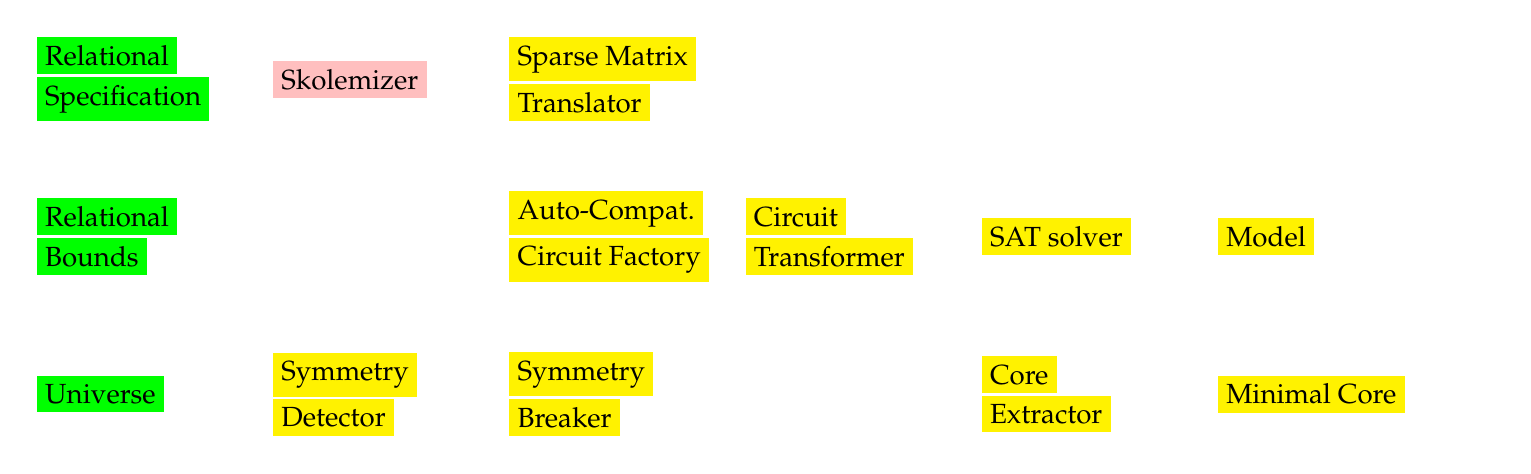
\begin{tikzpicture}
  \node (00)                   {\dtwo{Relational}{Specification}};
  \node (01) [below of=00
             ,yshift=\vshim]   {\dtwo{Relational}{Bounds}};
  \node (02) [below of=01
             ,yshift=\vshim]   {\done{Universe}};
  %% All these handled in parsing (get from user, interpret from syntax in parser)

  \node (10) [right of=00
             ,xshift=\hshim] {\sone{Skolemizer}};
  %% Skipping skolemizer, won't use existentials for now (performance implications?)

  \node (11) [right of=01
             ,xshift=\hshim] {};
  \node (12) [right of=02
             ,xshift=\hshim] {\todo{Symmetry}{Detector}};

  \node (20) [right of=10
             ,xshift=\hshim] {\todo{Sparse Matrix}{Translator}};
  \node (21) [right of=11
             ,xshift=\hshim] {\todo{Auto-Compat.}{Circuit Factory}};
  \node (22) [right of=12
             ,xshift=\hshim] {\todo{Symmetry}{Breaker}};

  \node (31) [right of=21
             ,xshift=\hshim] {\todo{Circuit}{Transformer}};
  \node (32) [right of=22
             ,xshift=\hshim] {};

  \node (41) [right of=31
             ,xshift=\hshim] {\tone{SAT solver}};
  \node (42) [right of=32
             ,xshift=\hshim] {\todo{Core}{Extractor}};

  \node (51) [right of=41
             ,xshift=\hshim] {\tone{Model}};
  \node (52) [right of=42
             ,xshift=\hshim] {\tone{Minimal Core}};



  %\draw (00) -- (10);
  %\draw (01) -- (10);
  %\draw (01) -- (12);
  %\draw (01) -- (20);
  %\draw (01) -- (22);
  %\draw (02) -- (12);

  %\draw (10) -- (20);
  %\draw (12) -- (22);

  %\draw (20) -- (21);
  %\draw (20) -- (31);
  %\draw (22) -- (21);
  %\draw (22) -- (31);

  %\draw (31) -- (41);

  %\draw (41) -- (42);
  %\draw (52) -- (41);
  %\draw (41) -- (51);
  %\draw (42) -- (52);
  %\draw (42) -- (41);

\end{tikzpicture}

\vspace{0.2cm}
\colorcode

\end{center}
\end{document}
